\section{\Large PROBLEM SET 7}

\subsection{Problem 1 - Introduce representative (from manufacturer or Wertz or first lectures) sensor errors in the form of constant bias and Gaussian noise with given standard deviation.}

Bias and Gaussian noise were first introduced to the startracker measurements through adding them to the unit vector that represented the location of an identified star in the ECI frame. Through analyzing star trackers produced by different manufacturers, the constant bias was set to 5 arcseconds and the mean of the Gaussian noise was set to 1 arcsecond based on the values given by Honeywell for their MST satellite. From there, the position vector of the star was converted to spherical coordinates so that the the noise and bias could be added to the angular components, $\theta$ and $\phi$. The bias was directly added to the unit vector, and the noise was added through multiplying the standard deviation by a a normal distribution with mean of zero and a standard deviation of one. The resultant simulink model and code for this are show below.

\begin{figure}[H]
    \centering
    \captionsetup{ justification = centering }
    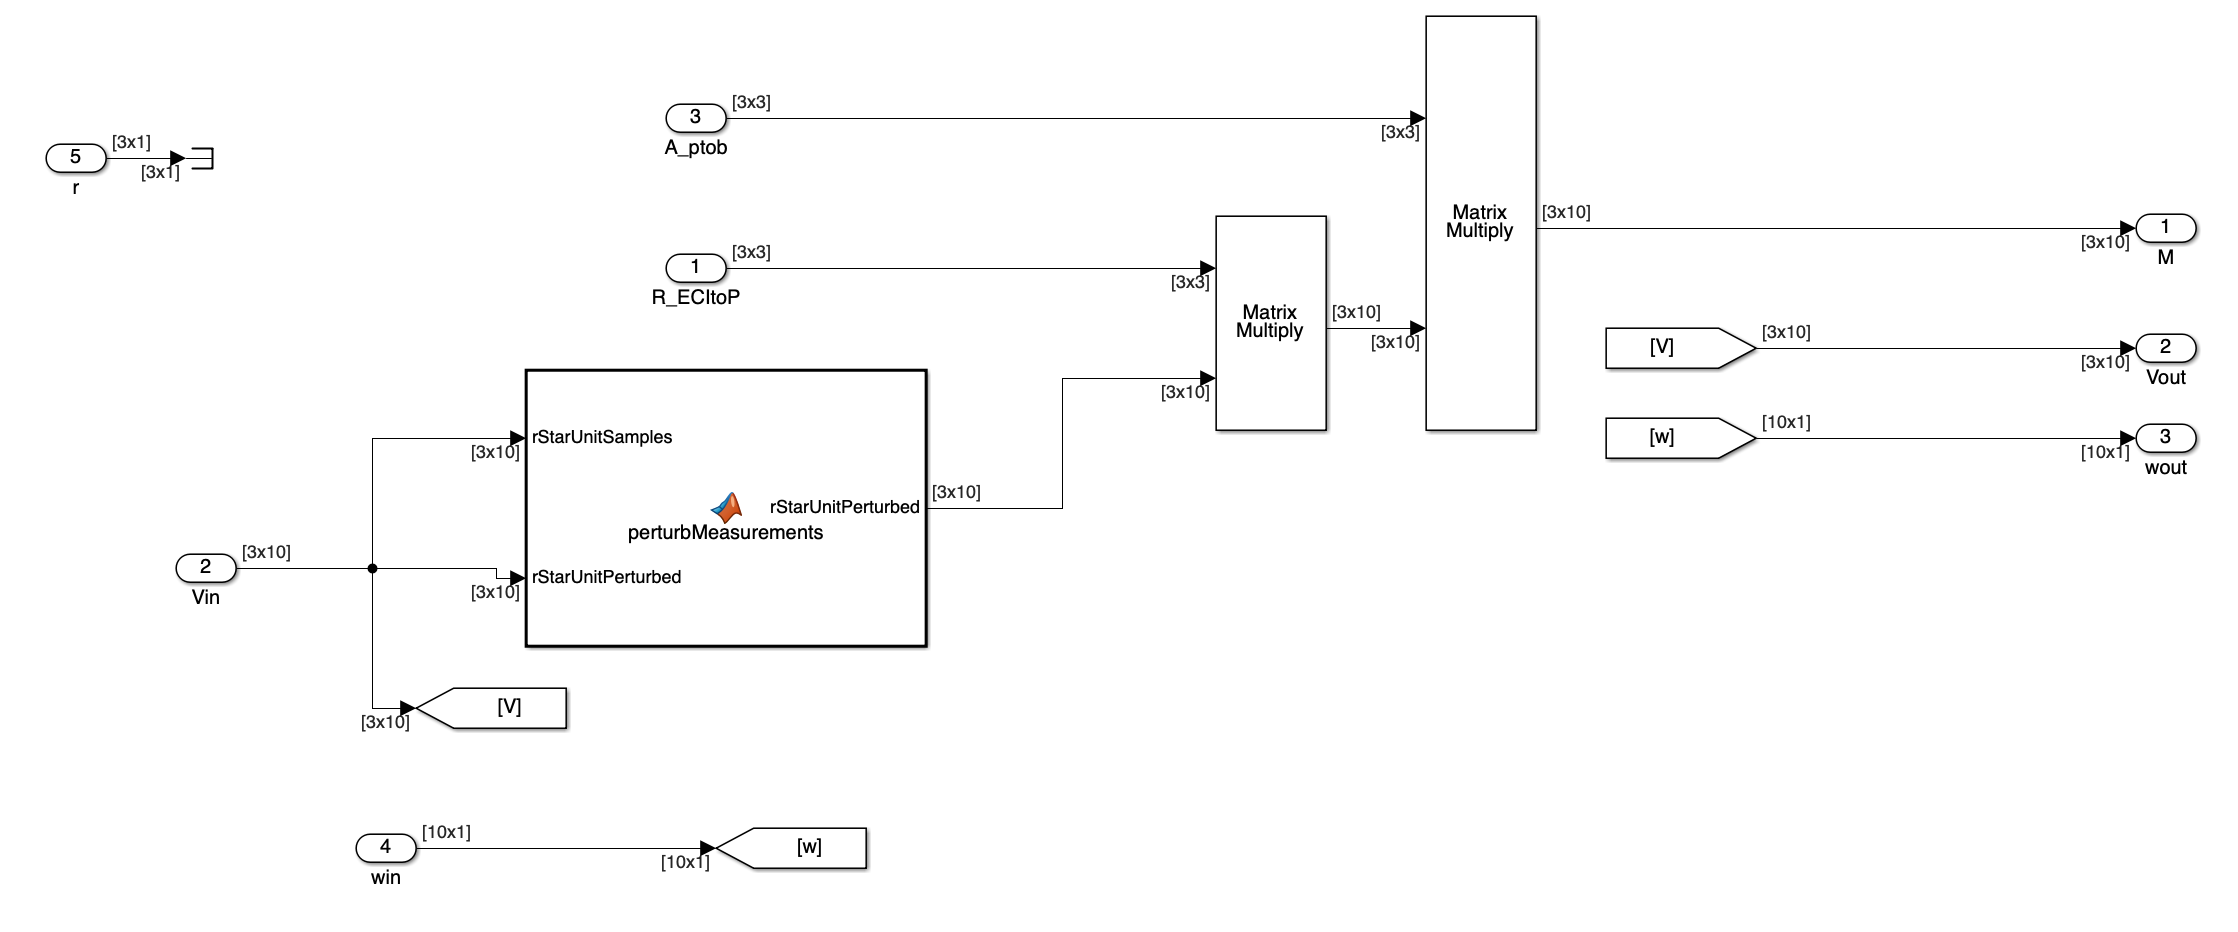
\includegraphics[width = 15cm]{Images/PS7/starTrackerErrorSimulink.png}
    \caption{Star Tracker Error Model in Simulink}
    \label{fig:starTrackerErrorSimulink}
\end{figure}

\begin{figure} [H]
    \centering
    \begin{lstlisting}
function rStarUnitPerturbed = perturbMeasurements(rStarUnitSamples, rStarUnitPerturbed)

% rStarUnitPerturbed = zeros(size(rStarUnitSamples));

% Bias and standard dev from known star tracker data (Honeywell MST)
mu = 5 * (pi / 180 / 3600); % Bias error in radians (converted from 5 arcseconds)
sigma = 1 * (pi / 180 / 3600); % Standard deviation of noise in radians (converted from 1 arcseconds)

nStars = length(rStarUnitSamples(1,:));

for i = 1:nStars

    % Get one star measurement
    rStarUnit = rStarUnitSamples(:,i);

    % Convert to spherical coordinates
    x = rStarUnit(1);
    y = rStarUnit(2); 
    z = rStarUnit(3);
    r = sqrt(x^2 + y^2 + z^2);
    theta = acos(z / r);
    phi = atan2(y, x);
    
    % Calculate the displacement due to bias error
    d_bias = mu;
    
    % Generate Gaussian noise and calculate displacement
    noise = sigma .* randn(1); % Angular noise in radians
    d_noise = noise;
    
    % Add the errors to the sperical coords
    theta_perturbed = theta + d_bias + d_noise;
    phi_perturbed = phi + d_bias + d_noise;
    
    % Convert back to spherical coordinates
    x_perturbed = r * sin(theta_perturbed) * cos(phi_perturbed);
    y_perturbed = r * sin(theta_perturbed) * sin(phi_perturbed);
    z_perturbed = r * cos(theta_perturbed);
    
    u_measured = [x_perturbed; y_perturbed; z_perturbed];
    
    % Normalize the measured vector to ensure it remains a unit vector
    u_measured = u_measured ./ norm(u_measured);

    rStarUnitPerturbed(:,i) = u_measured;
    
end
end
    \end{lstlisting}
    \caption{Star Tracker Noise}
    \label{fig:starTrackerNoise}
\end{figure}

For the $\omega$ error, the constant bias and the standard deviation of the Gaussian noise were once again pulled from a gyroscope manufacturer. This time they were pulled from Bosch Sensortec for the BMI160. The bias error was given as 3 $\degree$/$s$ and the standard deviation was set to  0.014 $\degree$/$\left(s \sqrt{Hz}\right)$. A bandwidth of one was assumed to convert the standard deviation to $\degree$/$s$. The standard deviation was then multiplied by a normal distribution with mean of zero and a standard deviation of one. The resultant simulink model and code are shown below.

\begin{figure}[H]
    \centering
    \captionsetup{ justification = centering }
    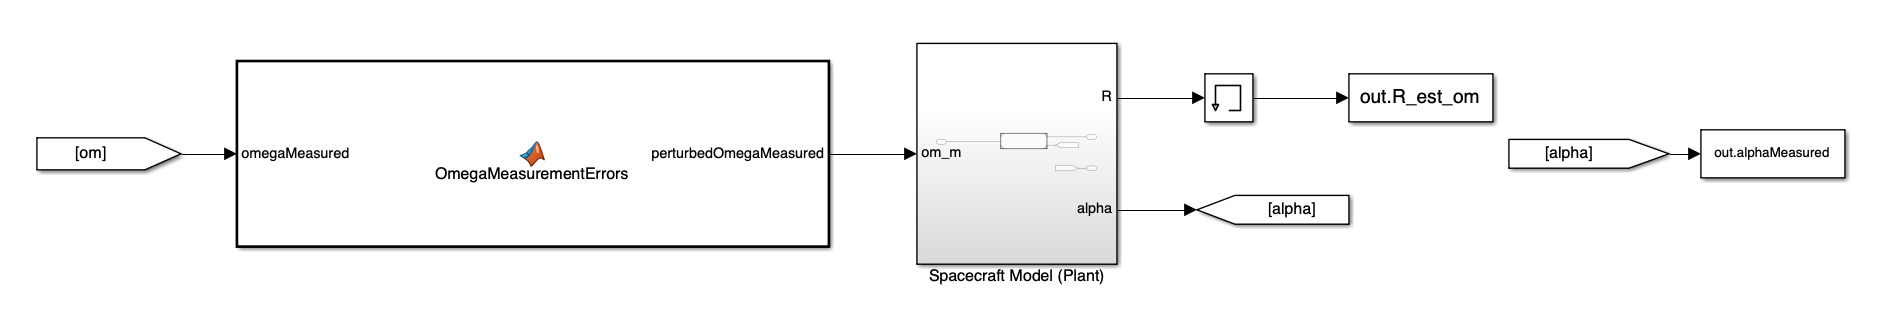
\includegraphics[width = 15cm]{Images/PS7/GyroErrorSimulink.png}
    \caption{Gyroscope Error Model in Simulink}
    \label{fig:gyroErrorSimulink}
\end{figure}

\begin{figure} [H]
    \centering
    \begin{lstlisting}
function perturbedOmegaMeasured = OmegaMeasurementErrors(omegaMeasured)

% Convert degrees per second to radians per second for bias error
bias_error_deg_per_sec = 3; % Example bias error in degrees per second (from Bosch BMI160)
bias_error_rad_per_sec = bias_error_deg_per_sec * (pi / 180); % Convert to radians per second

% Convert noise density to standard deviation for a given bandwidth
noise_density_deg_per_sec_sqrtHz = 0.014; % Example noise density in degrees per second per sqrt(Hz)
bandwidth = 1; % Assuming a bandwidth of 1 Hz for simplicity
noise_std_dev_deg_per_sec = noise_density_deg_per_sec_sqrtHz * sqrt(bandwidth); % Standard deviation in degrees per second
noise_std_dev_rad_per_sec = noise_std_dev_deg_per_sec * (pi / 180); % Convert to radians per second

% Bias error (constant offset)
bias_error = bias_error_rad_per_sec .* ones(size(omegaMeasured));

% Generate Gaussian noise
noise = noise_std_dev_rad_per_sec .* randn(size(omegaMeasured));


% Add the errors to the unit vector
error = bias_error + noise;
perturbedOmegaMeasured = error + omegaMeasured;
end
    \end{lstlisting}
    \caption{Gyroscope Noise}
    \label{fig:gyroNoise}
\end{figure}

\subsection{Problem 2 - Re-apply the attitude determination algorithms from the previous pset. Plot attitude estimation error. Note that the attitude estimation error represents a rotation matrix (DCM) which quantifies how far the estimated
attitude is from the true attitude. You can use any parameterization to plot the attitude estimation errors corresponding to this DCM. Is the result consistent with the sensor bias and noise you have introduced?}

The error for the "undersampled" (2 available measurement) case from the previous assignment was once again plotted for the star tracker measurements. In order to see the error that was present in addition to the numerical integration error, the constant bias and Gaussian noise were scaled by a factor of 1e3 to make the distinction clear. 

\begin{figure}[H]
    \centering
    \captionsetup{ justification = centering }
    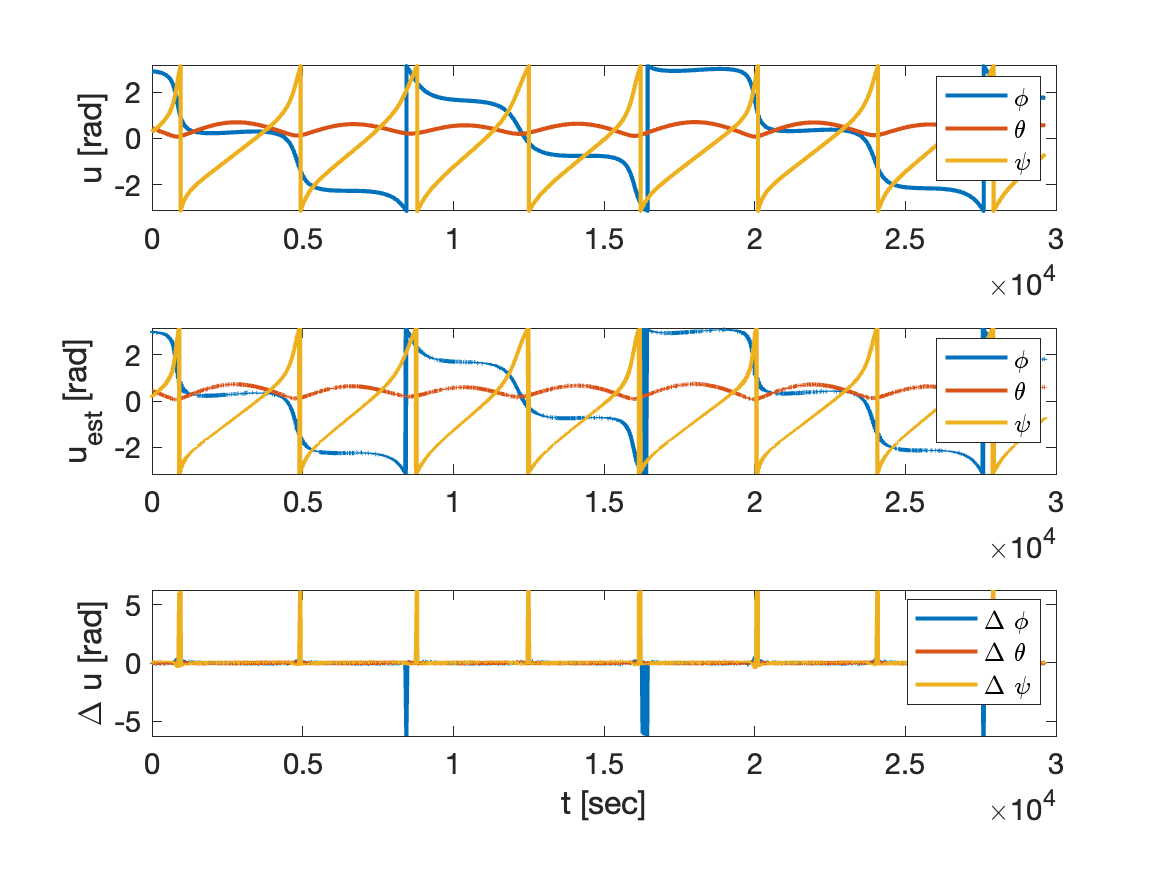
\includegraphics[width = 12cm]{Images/PS7/attitude_estimation_undersampled_det_default.png}
    \caption{Ground Truth vs. Estimated Attitude for Undersampled Deterministic Method with Feed Through Measurements with Noise and Bias}
    \label{fig:det_attitude_undersampled_default_noise}
\end{figure}

\begin{figure}[H]
    \centering
    \captionsetup{ justification = centering }
    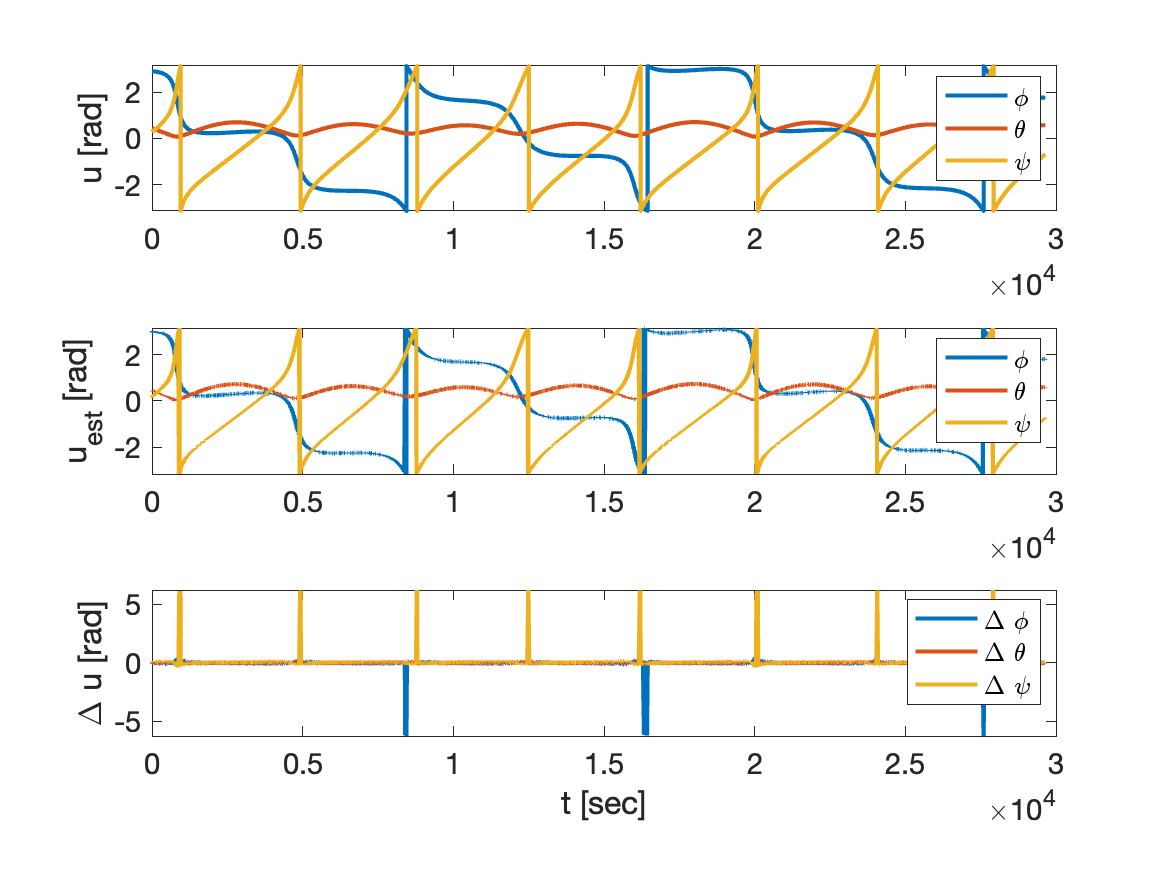
\includegraphics[width = 12cm]{Images/PS7/attitude_estimation_undersampled_det_fictitious.png}
    \caption{Ground Truth vs. Estimated Attitude for Undersampled Deterministic Method with Fictitious Measurements with Noise and Bias}
    \label{fig:det_attitude_undersampled_fictitious_noise}
\end{figure}

\begin{figure}[H]
    \centering
    \captionsetup{ justification = centering }
    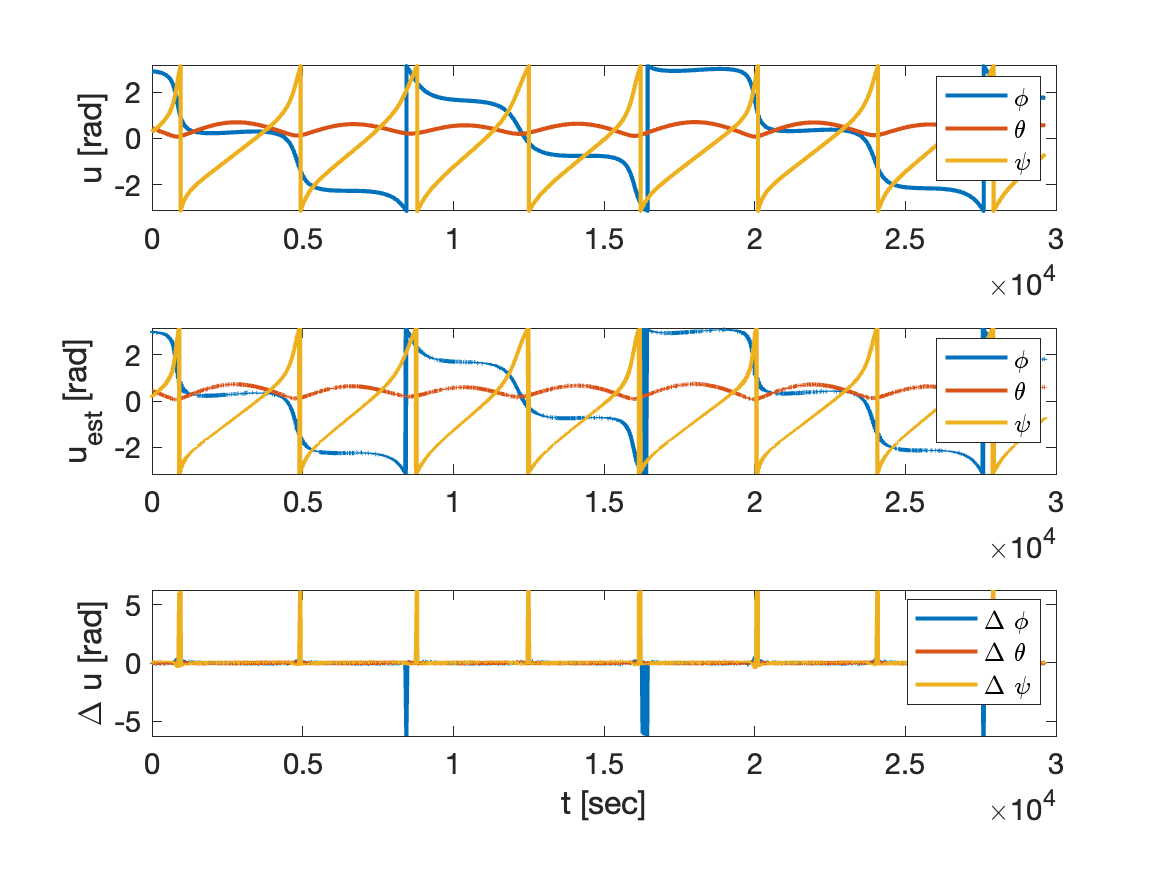
\includegraphics[width = 12cm]{Images/PS7/attitude_estimation_undersampled_q_default.png}
    \caption{Ground Truth vs. Estimated Attitude for Undersampled Statistical Method with Feed Through Measurements with Noise and Bias}
    \label{fig:stat_attitude_undersampled_default_noise}
\end{figure}

It can be seen in each of the plots that the added noise causes small oscillations in the measurements that aren't present in the ground truth values. These errors are small due to how accurate the star tracker measurements are but could still lead to issues if not properly accounted for.

For the $\omega$ measurements, Figure \ref{} was generated to show the error between the sensor and ground truth.




\subsection{Problem 3 - For small sensor errors, the DCM corresponds to a small rotation. Can you give an interpretation of small angles (e.g., in Euler angles and quaternions) to the obtained error DCM?}

\subsection{Problem 4 - Start modeling actual sensors in dedicated (Simulink or otherwise) subsystems which are part of the spacecraft. These models take inputs from ground-truth simulation and provides output measurements, including systematic and random errors. Take inspiration from overview of sensors discussed in class and
textbook for typical errors.}

\subsection{Problem 5 - Designing and implement the time update of a KF/EKF to obtain the best estimate of the state from the available measurements and models:}

\subsubsection{Search in literature, define, and code a state transition matrix $\Phi$ which provides your state at step k+1 based on the state at step k. Verify that the output of this propagation step is consistent with the rigorous propagation of the attitude (numerical integration). Plot propagation errors as needed.}

For a Multiplicative Extended Kalman Filter (MEKF), the absolute attitude of the spacecraft is represented using a quaternion parameterization. This helps avoid singularities, while introducing the unitary norm constraint. To sidestep this issue, the state that is actually fed through the filter itself consists of a 3-component vector that represents a small deviation between a reference quaternion at the previous timestep and the reference quaternion for the current timestep. The expected value of these values is zero, and this component of the state is only altered during the measurement update. As a result, the time update step of MEKF will not update this value. The full state vector also contains the three angular velocity of the spacecraft about its principal axes. The full state vector can be written as seen in Equation \ref{eq:kf_state_def}.

\begin{equation} \label{eq:kf_state_def}
    \vec{x} = \begin{bmatrix}
        \alpha_1 \\ \alpha_2 \\ \alpha_3 \\ \omega_x \\ \omega_y \\ \omega_z
    \end{bmatrix}
\end{equation}

The discrete state transition matrix for this state in the time update is shown below in Equation \ref{eq:kf_statetrans_block}.

\begin{equation} \label{eq:kf_statetrans_block}
    \boldsymbol{\Phi}_t = \begin{bmatrix}
        \boldsymbol{\Phi}_{\alpha,t} & 0 \\
        0 & \boldsymbol{\Phi}_{\omega,t}
    \end{bmatrix}
\end{equation}

Where $\boldsymbol{\Phi}_{\alpha,t}$ and $\boldsymbol{\Phi}_{\omega,t}$ are defined in Equations \ref{eq:alpha_STM} and \ref{eq:omega_STM}.

\begin{equation} \label{eq:alpha_STM}
    \boldsymbol{\Phi}_{\alpha,t} = \boldsymbol{I} + s_{\omega} \boldsymbol{\left[ \vec{\omega} \times \right]} + \left( \frac{1 - c_{\omega}}{\omega ^2} \right) \boldsymbol{\left[ \vec{\omega} \times \right]} \boldsymbol{\left[ \vec{\omega} \times \right]}
\end{equation}

\begin{equation} \label{eq:omega_STM}
    \Phi_{\omega,t} = \boldsymbol{I} + \begin{bmatrix}
        0 & \frac{I_y - I_z}{I_x} \omega_{z,t} & \frac{I_y - I_z}{I_x} \omega_{y,t} \\
        \frac{I_z - I_x}{I_y} \omega_{z,t} & 0 & \frac{I_z - I_x}{I_y} \omega_{x,t} \\
        \frac{I_x - I_y}{I_z} \omega_{y,t} & \frac{I_x - I_y}{I_z} \omega_{x,t} & 0
    \end{bmatrix} \frac{\Delta t}{2}
\end{equation}

Where

\begin{equation*}
    \omega \triangleq \Vert \vec{\omega} \Vert
\end{equation*}
\begin{equation*}
    c_{\omega} \triangleq \cos{\frac{\omega \Delta t}{2}}
\end{equation*}
\begin{equation*}
    s_{\omega} \triangleq \frac{1}{\omega} \sin{\frac{\omega \Delta t}{2}}
\end{equation*}



\subsubsection{Search in literature, define, and code a control input matrix B which provides the increment to your state at step k+1 due to a control torque at step k. Hint: optional at this stage since you do not have a controller yet.}


\subsubsection{(a) and (b) allow you to propagate the state from k to k+1 including the known control input torques. Hint: Initially you will design the filter by neglecting any control torque from your simulation.}

\subsubsection{Define and code an initial state error covariance matrix P which quantifies the uncertainty of your initial state. This can be picked as diagonal matrix with diagonal elements representing the variance of each state parameter $\sigma ^2$. Initially you can neglect cross-covariance terms assuming that errors of various state components are not correlated.}

\subsubsection{The time update of the EKF needs $\Phi$, B, and P. Hint: You could increment your navigation performance by keeping the filter receptive to new measurements at steady state through the addition of constant process noise Q at each step. Initially you can define Q similar to P but much smaller (e.g., 1/10 or 1/100).}

\subsection{Problem 6 - Produce plots showing true attitude estimation errors (estimate vs truth with statistics), formal or estimated attitude estimation errors (covariance from filter). Discuss the results, do they meet expectations? How well is the true estimation error described by the formal covariance? Note that we are only implementing the time update even if we call them “attitude estimates and estimation errors”.}